%%**************************************************************
%% Vorlage fuer Bachelorarbeiten (o.ä.) der DHBW
%%
%% Autor: Tobias Dreher, Yves Fischer
%% Datum: 06.07.2011
%%**************************************************************

\newcommand{\pdftitel}{Entwicklung eines Web Based Training Systems nach einem Lernmodell}
\newcommand{\autor}{Michael Gruben \& Julian Babics \& Benjamin Merkle}
\newcommand{\arbeit}{Studienarbeit}

\input{ads/header} 

% Ab jetzt können auch Umlaute verwendet werden
\newcommand{\titel}{\pdftitel}
\newcommand{\martrikelnr}{2788654}
\newcommand{\kurs}{TAI10B1}
\newcommand{\datumAbgabe}{Mai 2013}
\newcommand{\firma}{M+M, Medical Solutions, SAP AG}
\newcommand{\firmenort}{Pforzheim, Karlsruhe, Roth}
\newcommand{\abgabeort}{Karlsruhe}
\newcommand{\abschluss}{Bachelor of Science}
\newcommand{\studiengang}{Studienganges Angewandte Informatik}
\newcommand{\dhbw}{Karlsruhe}
\newcommand{\betreuer}{Dr. Kay Margareth Berkling}
\newcommand{\gutachter}{Prof. Dr. Johannes Freudenmann}
\newcommand{\zeitraum}{2,5 Monate}
\newcommand{\arbeitsart}{\arbeit}

\makeglossaries
\input{ads/glossary}

\begin{document}

	% Deckblatt
	\begin{spacing}{1}
		\begin{titlepage}
	\begin{longtable}{p{.55\textwidth} p{.85\textwidth}}
	  {} & 
	  {\includegraphics[height=2.6cm]{dhbw.png}}
	\end{longtable}
	\enlargethispage{20mm}
	\begin{center}
	  \vspace*{12mm}	{\LARGE\bf \titel }\\
	  \vspace*{12mm}	{\large\bf \arbeit}\\
	  \vspace*{12mm}	für die Prüfung zum\\
	  \vspace*{3mm} 	{\bf \abschluss}\\
	  \vspace*{12mm}	des \studiengang\\
	  \vspace*{3mm} 	an der Dualen Hochschule Baden-Württemberg \dhbw\\
	  \vspace*{12mm}	von\\
	  \vspace*{3mm} 	{\large\bf Michael Gruben \normalsize\rm Meyle+Müller
	  GmbH+Co.KG (Pforzheim) \phantom{iiiiibH (Bruchsal)     }\&}\\
	  \vspace*{3mm} 	{\large\bf Julian Babics \normalsize\rm MedicalCommunications
	  Soft- und Hardware GmbH (Bruchsal) \&}\\
	  \vspace*{3mm} 	{\large\bf Benjamin Merkle \normalsize\rm SAP AG (Walldorf)
	  \phantom{mniiiiiiiiiiiiiiiiiiiiiiiiiiiiiiiiiiiiibH (Bruchsal)}}\\
	  \vspace*{12mm}	\datumAbgabe\\
	\end{center}
	\vfill
	\begin{spacing}{1.2}
	\begin{tabbing}
		mmmmmmmmmmmmmmmmmmmmmmmmmm     \= \kill
		\textbf{Bearbeitungszeitraum}  \>  \zeitraum\\
		%\textbf{Matrikelnummer, Kurs}  \>  \martrikelnr, \kurs\\
		%\textbf{Ausbildungsfirmen}      \>  Meyle+Müller GmbH+Co.KG (Pforzheim)\\
		%\>MedicalCommunications Soft- und Hardware GmbH (Bruchsal)\\
		%\>SAP Deutschland AG & Co. KG (Walldorf)\\
		\textbf{Betreuer}              \>  \betreuer\\
 		\textbf{Gutachter}             \>  \gutachter
	\end{tabbing}
	\end{spacing}
\end{titlepage}
	\end{spacing}
	\newpage

\renewcommand{\thepage}{\Roman{page}}
	\setcounter{page}{1}
	
	% Sperrvermerk
% 	\input{ads/sperrvermerk}
% 	\newpage
	
	% Erklärung
	\thispagestyle{empty}

\section*{Erklärung}
% http://www.se.dhbw-mannheim.de/fileadmin/ms/wi/dl_swm/dhbw-ma-wi-organisation-bewertung-bachelorarbeit-v2-00.pdf
\vspace*{2em}

Wir erklären hiermit ehrenwörtlich: \\
\begin{enumerate}
\item dass wir unsere {\arbeitsart} mit dem Thema
{\itshape \titel } ohne fremde Hilfe angefertigt haben;
\item dass wir die Übernahme wörtlicher Zitate aus der Literatur sowie die
Verwendung der Gedanken anderer Autoren an den entsprechenden Stellen innerhalb
der Arbeit gekennzeichnet haben;
\item dass wir meine {\arbeitsart} bei keiner anderen Prüfung vorgelegt haben;
\item dass die eingereichte elektronische Fassung exakt mit der eingereichten schriftlichen Fassung
übereinstimmt.
\end{enumerate}

Wir sind uns bewusst, dass eine falsche Erklärung rechtliche Folgen haben wird.

\vspace{3em}

\abgabeort, \datumAbgabe
\vspace{4em}

\autor \newpage \thispagestyle{empty}
\selectlanguage{english}Copyright (C)  2013  Michael Gruben, Julian
Babics, Benjamin Merkle.

Permission is granted to copy, distribute and/or modify this document under the
terms of the GNU Free Documentation License, Version 1.3 or any later version
published by the Free Software Foundation; with no Invariant Sections, no
Front-Cover Texts, and no Back-Cover Texts. A copy of the license is included in
the section entitled "GNU Free Documentation License".
\selectlanguage{ngerman}
	\newpage

	% Abstract
	\pagestyle{empty}

\renewcommand{\abstractname}{Zusammenfassung}

\begin{abstract}
Im Verlauf der Bearbeitung der Studienarbeit "`Analyse und Vergleich von
Autorensystemen für ein WBT zu Vorlesungsinhalten"' ist in der Vorlesung
"`Gamification"' ein Konzept für ein WBT\footnote{Web Based Training}-System
entstanden. Aus dieser Vorstellung ist die Idee, und damit die Motivation der
Studienarbeit, entstanden es in die Realität umzusetzen.

Es handelt sich um eine Webapplikation, die diverse WBTs in entsprechenden
Kategorien zum Bearbeiten anbietet. Das Lernmodell der Gebrüder Dreyfuß
wird in diese verwoben. In dem Modell wird die Kompetenz in einem Fachgebiet auf
zwei unterschiedlichen Ebenen betrachtet, die fachliche Kompetenz und die
Fähigkeit erklären zu können.

Zunächst wird die fachliche Kompetenz betrachtet. Demnach bearbeitet ein Neuling
auf dem ersten Kompetenzlevel eines bestimmten Fachbereiches ein grundlegendes
WBT, dessen abschließende Fragen nach vorgegebenen Schemata und grundlegender
Eigenschaften beantwortet werden. Ein Experte auf dem vierten Kompetenzlevel
muss hingegen Antworten auf Fragen wissen, die ein wesentlich komplexeres
Verständnis eines Sachverhaltes verlangen.

Um seine Fähigkeit erklären zu können unter Beweis zu stellen, engagiert man
sich mit Hilfestellungen für niedere fachliche Level. Beurteilen diese die
Hilfestellung als gut, kann der Mastery Rang erreicht werden, der sich noch über
dem Experten befindet. Nach dem Dreyfuß-Modell dürfen sich Lernender und
Lehrender durch maximal zwei Level unterscheiden. Der Mastery-Level ist hingegen
ein "`erklärender Experte"', der nicht nur fachlich höchst Kompetent ist,
sondern auch sehr gut auch für einen Anfänger erklären kann, ohne in fachliche
Details abzuschweifen.

Das WBT-System, welches beide beschriebenen Ebenen der Kompetenz organisiert,
wird unter einer freien Lizenz veröffentlicht werden. So kann das als noch sehr
simpel und eingeschränkt erwartete Ergebnis der Studienarbeit als Community
Projekt weiterleben und weiterentwickelt werden. Bereits vor Bearbeiten der
Studienarbeit wird damit gerechnet, das nur ein kleiner und spezieller aber
funktionaler Teil des Konzeptes umgesetzt werden wird. Der Fokus liegt
dabei grundsätzlich mehr auf Funktionalität, einer leicht zu erweiternden
Architektur der Software und einem benutzerfreundlichem Interface, als auf
einem gut aussehendem Design.
\end{abstract}
% \begin{abstract}
% Ein Abstract ist eine prägnante Inhaltsangabe, ein Abriss ohne
% Interpretation und Wertung einer wissenschaftlichen Arbeit. In DIN
% 1426 wird das (oder auch der) Abstract als Kurzreferat zur
% Inhaltsangabe beschrieben.
% 
% \begin{description}
% \item[Objektivität] soll sich jeder persönlichen Wertung enthalten
% \item[Kürze] soll so kurz wie möglich sein
% \item[Genauigkeit] soll genau die Inhalte und die Meinung der Originalarbeit wiedergeben
% \end{description}
% 
% Üblicherweise müssen wissenschaftliche Artikel einen Abstract
% enthalten, typischerweise von 100-150 Wörtern, ohne Bilder und
% Literaturzitate und in einem Absatz.
% 
% Quelle \url{http://de.wikipedia.org/wiki/Abstract} Abgerufen 07.07.2011
% \end{abstract}
% 
% 
% \renewcommand{\abstractname}{Summary}
% \begin{abstract}
% An abstract is a brief summary of a research article, thesis, review,
% conference proceeding or any in-depth analysis of a particular subject
% or discipline, and is often used to help the reader quickly ascertain
% the paper's purpose. When used, an abstract always appears at the
% beginning of a manuscript, acting as the point-of-entry for any given
% scientific paper or patent application. Abstracting and indexing
% services for various academic disciplines are aimed at compiling a
% body of literature for that particular subject.
% 
% The terms précis or synopsis are used in some publications to refer to
% the same thing that other publications might call an "abstract". In
% management reports, an executive summary usually contains more
% information (and often more sensitive information) than the abstract
% does.
% 
% Quelle: \url{http://en.wikipedia.org/wiki/Abstract_(summary)}

% \end{abstract}

	\newpage

	\pagestyle{plain}

	% Inhaltsverzeichnis
	\begin{spacing}{1.1}
		\setcounter{tocdepth}{2}
		\tableofcontents
	\end{spacing}
	\newpage

	\setglossarysection{chapter}
	% Abkürzungsverzeichnis
	% vorher in Konsole folgendes aufrufen: 
	%	makeglossaries makeglossaries dokumentation.acn && makeglossaries dokumentation.glo
	%\printglossary[type=\acronymtype,title=Abkürzungsverzeichnis,toctitle=Abkürzungsverzeichnis]
	\cleardoublepage
	\phantomsection \label{listofacs}
	\addcontentsline{toc}{chapter}{Abkürzungsverzeichnis}
	\chapter*{Abkürzungsverzeichnis}

\begin{acronym}[WYSIWYG]
\newcommand{\acrov}{\vspace{\parsep}}
\setlength{\itemsep}{-\parsep}
\acro{ADL}{Advanced Distributed Learning}
\acro{AGPL}{Affero GNU General Public License}
\acro{API}{Application Programming Interface}
\acrov
\acro{CAM}{Content Aggregation Model}
\acro{CBT}{Computer Based Training}
\acrov
\acro{DE}{Distance Education}
\acro{DRY}{Don't repeat yourself}
\acrov
\acro{F2F}{Face-To-Face}
\acrov
\acro{GPL}{GNU General Public License}
\acro{GUI}{Graphical User Interface}
\acrov
\acro{KISS}{Keep it simple stupid'}
\acrov
\acro{LMS}{Learning Management System}
\acrov
\acro{MVC}{Model View Control}
\acrov
\acro{OE}{Online Education}
\acrov
\acro{PIF}{Package Interchange File}
\acrov
\acro{RTE}{Run Time Environment}
\acrov
\acro{SCO}{Shared Content Object}
\acro{SCORM}{Shared Content Object Reference Model}
\acrov
\acro{WBT}{Web Based Training}
\acro{WYSIWYG}{What You See Is What You Get}
\acrov
\acro{YAGNI}{You ain't gonna need it}
\end{acronym}

	% Glossar
	\printglossary[style=altlist,title=Glossar]
	
	\newpage
		
	\renewcommand{\thepage}{\arabic{page}}
	\setcounter{page}{1}
	
	% Inhalt
	\chapter{Einleitung}\label{ref:chaptIntroduction}
Basierend auf der Studienarbeit "`Analyse von Authorensystemen für ein WBT zu
Vorlesungszwecken von Michael Gruben \cite{gruben:2012} wird in dieser
Studienarbeit ein System aus \ac{WBT}s geschaffen. Das Konzept für das
Produkt des Projektes ist im Rahmen der Vorlesung "`Gamification"' entstanden.

Dabei handelt es sich grundsätzlich um eine Blended Learning Plattform, die
interessierten Lernenden eine zentrale Anlaufstelle bietet. Es werden also
eLearning und persönliches Lernen miteinander kombiniert. Umrahmt und
gamifiziert wird die Idee mithilfe des Dreyfus fünf Etappen Modells mentaler
Aktivitäten. Die in dieser Studienarbeit verwendeten Bezeichnungen unterliegen
gegebenenfalls weiteren Änderungen und sind für die deutschsprachige Version der
Plattform bestimmt.

Inhalte der vorligenden Studienarbeit sind Einblicke in die Entwicklung des
ersten Prototyps. Dazu zeigt Kapitel \ref{ref:chaptConcept} die Konzeption und
damit die grundlegende Idee der Architektur. Daran anschließend wird in Kapitel
\ref{ref:chaptScript} näher auf den tatsächlichen Entwurf eingegangen. Hier
wird konkret auf Klassen und Methoden eingegangen, welche die Realisierung
bestimmter Use-Cases zum Ziel haben. Kapitel \ref{ref:chaptImplementation}
zeigt, wie der Entwurf letztlich realisiert wird. Hier sind auch erste
Screenshots der Anwendung zu sehen. Um die vorrangegangenen Schritte
zusammenzufassen und kurz auszuwerten, gibt Kapitel \ref{ref:chaptConclusion}
einen Gesamtüberblick. Darauf aufbauend bietet Kapitel \ref{ref:chaptSummary}
eine Auswertung, die alle Aspekte des Projekts umfasst. Zusätzlich werden hier
Ausblicke auf die weitere Verwendung des Projektergebnisses gegeben.

Am Ende des Projekts steht ein funktionierender Prototyp, der die
wesentlichen Funktionen beherrscht. Weiterhin wird ein Konzept entwickelt worden
sein, welches das Projekt an zentralen Stellen bekannt macht und so für eine
rege Beteiligung sorgen soll. Mit der Namensgebung "`Masterly Mate"' wurde
bereits vor dem eigentlichen Projektstart ein wesentlicher Schritt zur
Bekanntmachung getan.
	\part{Vorbereitungen}
	\chapter{Projektplanung}
Die Projektidee entstammt von studentischer Seite. In Abbildung
\ref{ref:wolkeMM} ist eine Wortwolke zu sehen, in der in Stichworten beschrieben
ist, was sich unter Masterly Mate vorzustellen ist.

\begin{figure}[H]
\includegraphics[width=1\textwidth]{MasterlyMateWolke.png}
\caption{Wortwolke über die "`Masterly Mate"'-Idee}\label{ref:wolkeMM}
\end{figure}

Das Projekt nimmt sich eine Art Lernplattform zum Ziel, auf der Lernende auf
Lehrende treffen sollen. Dabei entstehen Situationen, in der eine lehrende
Person zu einer lernenden wird, und umgekehrt. Es sollen Diskussionen über
bestimmte Fachgebiete stattfinden können und ideale Tutoren für bestimmte
Fragestellungen gefunden werden. Da es nichts zu gewinnen gibt, engagiert sich
jeder Teilnehmer freiwillig. Er erhält Wissen und kann dieses im nächsten Moment
an weitere interessierte Personen weitergeben, was sein eigenes Wissen erneut
festigt. Lehrstunden sollen im gemütlichen Umfeld, wie Caffees oder Parks
stattfinden. Masterly Mate bietet dazu eine regionale Suche an, mit deren Hilfe
Lernende und Lehrende aufeinander treffen. Dem Duo steht es auch offen auf
andere Kommunikationskanäle, wie Chat oder E-Mail, zu wechseln. Jeder Nutzer
kann als Tutor für sein Fachgebiet oder seine Fachgebiete fungieren.

Um stets einen idealen Tutor zu finden, folgt die Idee dem Dreyfus fünf Etappen
Modell mentaler Aktivitäten, welches in Abschnitt \ref{ref:dreyfus} näher
beschrieben wird. So ist gewährleistet, dass ein Neuling die Inhalte von einer
Person erklärt bekommt, die selbst noch im Lernprozess steckt und es können
Inhalte, Tipps und Hinweise auf passendem Niveau ausgetauscht werden.

Letztlich soll das Ziel der Mitgliedschaft auf der Plattform nicht sein, der
beste Guru eines Faches zu werden oder der beste Lehrer zu werden. Es geht darum
Teil einer Bildungsgemeinschaft zu sein und sich gegenseitig engagiert zu
unterstützen.

\section{Motivation und Notwendigkeit}\label{ref:projectMotivation}
Die Motivation zu dieser Idee entstand aus der interessanten und
erwartungsvollen Kombination von eLearning und Gamification. Hinzu kommt die
heute populäre Vorstellung von Blended Learning, wodurch das doch sehr trockene
und eintönige Durcharbeiten von WBTs durch Lehreinheiten mit einem Tutor
unterstützt wird.

Masterly Mate soll eine zentrale Anlaufstelle für diverse Weiterbildungs- und
Lernangelegenheiten sein. Unabhängig davon, ob die Motivation privatem Interesse
oder dem eigenen Bildungsweg entspringt, soll jeder Interessent wissen, dass
die Plattform Antworten bietet.

Die Notwendigkeit resultiert aus der fehlenden Fähigkeit des Internets,
Sachverhalte erläutern zu können. Heute ist es Usus beim Recherchieren das
Internet zu gebrauchen, in dem rohe Daten und Informationen vorliegen. Wissen
ist dort eher rar. Es gibt bisher nur wenige Plattformen, wie Wikipedia, die
existieren, um Wissen zu publizieren, jedoch fehlt auch dort eine erklärende und
erläuternde Komponente durch einen Menschen. Dieses Manko soll Masterly Mate
ausgleichen.

\section{Abgrenzung}
Das Projektergebnis behauptet keinen Anspruch auf ein vollwertiges \ac{LMS}. Es
fehlt die Komponente zur Organisation kompletter Lernpakete. In Masterly Mate
stehen die WBTs unabhängig da. Sie sind allein Mittel zum Zweck als Beleg für
die fachliche Kompetenz.

Weiterhin soll es Wikipedia nicht ersetzen. Das Projektergebnis bietet keine
ausformulierten Texte oder Artikel zu Lerninhalten. Der Fokus liegt wesentlich
stärker auf der Komponente Wissen zu vermitteln.

\section{Zielsetzung}
Da das Projekt insgesamt auf einen längeren Zeitraum angesetzt ist, lässt es
sich nicht innerhalb der Bearbeitungszeit der vorliegenden Studienarbeit
umsetzen. Aus diesem Grund sind die Ziele zum einen in operative und zum anderen
in strategische zu unterteilen. 

\subsection{Operative Ziele}
Wie in Kapitel \ref{ref:chaptIntroduction} bereits angerissen wurde, soll zu
Projektende ein funktionaler Prototyp stehen. Auch ist ein Konzept angedacht,
welches der Bekanntmachung von Masterly Mate dient. Eventuell wird sich bis
dahin eine kleine, lebendige Gemeinschaft gebildet haben, die die Plattform
nutzt und um Inhalte erweitert. Die ersten Nutzer sollen automatisch unabhängig
ihres didaktischen Grades\footnote{näher erläutert in Abschnitt
\ref{ref:rankTeach}} Autoren sein. So ist gewährleistet, dass Inhalte für neue
Nutzer bereits existieren. 

Das Projekt als Ganzes soll einen leichten Start haben. Sind die Ziele für die
ersten Nutzer zu hoch gesteckt, resultiert aus der geringen Anzahl von Nutzern
und der damit schwer erreichbaren nächsten Rängen Frustration und Unwille zur
Nutzung der Plattform. Somit ist angedacht, die erforderliche Punktzahl für
höhere Ränge (siehe Abschinitt \ref{ref:dreyfus}) mit der Menge der Nutzer zu
skalieren.

\subsection{Strategische Ziele}
Längerfristig betrachtet soll eine rege und große Gemeinschaft entstehen, die
Hilfsbereitschaft nicht scheut. Dazu wird bereits zu Beginn der Entwicklung eine
Internationalisierung\footnote{siehe Abschnitt \ref{ref:internationalisierung}}
berücksichtigt. Masterly Mate soll zur, in Abschnitt \ref{ref:projectMotivation}
beschriebenen, zentralen Anlaufstelle heranwachsen.

Dabei werden, um den Reiz am Lernen zu erhöhen, mit der Menge der Nutzer die
Anforderungen für die jeweils nächsten Ränge erhöht. Denn je mehr Beteiligung
die Plattform erfährt, desto wahrscheinlicher ist es, einen Tutor in der
jeweiligen Region zu finden. Damit wird es auch immer einfacher, Punkte für den
didaktischen Rang zu sammeln.

\section{Lizensierung}
Für die Lizensierung wird auf die \ac{AGPL} zurückgegriffen. Dadurch ist eine
eventuelle Verbreitung der Software im Sinne von OpenSource gewährleistet. Die
AGPL ist kompatibel mit der \ac{GPL}. Dadurch ist sichergestellt, dass das
Projekt auch auf andere Lizenzen übertragen werden kann \cite{fsf:2007}.

Aus der Verwendung der AGPL entsteht die Pflicht, den Quelltext der Anwendung
direkt als Download anzubieten.

	\chapter{Theoretische Grundlagen}
Das Projekt basiert auf einigen theoretische Grundlagen. Dazu zählen
Lerntheorien und technische Begriffe, deren Erläuterungen Inhalt
dieses Kapitels sind. Dabei handelt es sich um eine Kurzfassung der
Beschreibungen aus \cite{gruben:2012}.

\section{Lernen}
Das Lernen selbst wird heute als ein Prozess verstanden. Dabei wirken "`mehrere
zentrale psychologische Phänomene (Motivation, Emotion,
Kognition)"'\cite{niegemann:2004} zusammen. 

Der Lernprozess besteht dabei aus drei Abschnitten:
\begin{enumerate}
  \item Zunächst werden Eindrücke wahrgenommen. Dabei tragen neue oder
  vergessene Eindrücke zur Umstrukturierung im Gehirn bei.
  \item Umstrukturieren bedeutet, dass Synapsen bewegt und andere Gehirnzellen
  angekoppelt werden.
  \item Mit Wiederholungen wird Wissen persistiert. Es entstehen stabile
  Strukturen, welche einfach und schnell abrufbar sind.
\end{enumerate}
In Abbildung \ref{pic:structSyn} wird diese Umstrukturierung illustriert
\cite{spitzer:2012}.

Von ein LMS wird erwartet, dass es diesen Lernprozess unterstützt. Anfänger
sollen die Möglichkeit erhalten zunächst klein anzufangen und die Grundlagen
eines bestimmten Sachverhaltes kennenzulernen. Fortschreitend können die
Anforderungen und Herausforderungen gesteigert werden, um den Lernprozess zu
unterstützten und zugleich die Motivation aufrecht zu erhalten.

\begin{figure}[H]
\centering
\includegraphics[width=0.7\textwidth]{SPIsynapseS50.png}
\caption{Umstrukturierung von Synapsen \footnotemark}\label{pic:structSyn}
\end{figure}\footnotetext{aus \cite{spitzer:2012}}

\section{Motivation}
Die Motivation ist ein wesentliches Standbein des Lernprozesses. Fehlt sie, so
ist es für Lernende bedeutend erschwert, Lerninhalte aufzunehmen, zu verarbeiten
und zu verstehen. Mithilfe von Motivation wird ein charakteristisches Verhalten
an den Tag gelegt, welches den Lernprozess aufrecht erhält \cite{jacobs:2010}.

Im Mittelpunkt jeder Motivation steht stets das persönliche Glück
\cite{stampfl:2012}. Dabei stehen Mittel zur Verfügung, die dem Lernenden auf
unterschliedliche weise unterstützen zu verstehen. Er kann zum einen
intrinsisch und zum anderen extrinsisch motiviert werden.

\subsection{Intrinsische Motivation}\label{ref:intrinsischeMotivation}
Die intrinsische Motivation wird auch als direkte Motivation bezeichnet. Damit
wird der Lernende direkt angesprochen und in seinen Bedürfnissen befriedigt und
seinen Wünschen wird unmittelbar nachgegangen. Ein intrinsisch motivierter
Lernender geht einer Tätigkeit im eigenen Interesse nach, es sind keine externen
Einflüsse nötig, die ihn zu seinen Handlungen erst bewegen müssen
\cite{jacobs:2010}.

Jede Lernsoftware hat aus dem zuvor erwähnten Sachverhalt die intrinsiche
Motivation zum Ziel. Dazu werden nicht selten unter Anderem auch gamifizierende
Inhalte verwendet (siehe \ref{ref:gamification}).

\subsection{Extrinsische Motivation}
Die andere Seite der Motivation kommt von aussen. Es werden Belohnungen gegeben
oder Strafe und negative Konsequenzen vermieden. Synonyme sind demnach
"`indirekte Motivation"', das "`Butterbrot-und-Peitsche-Prinzip"' oder
"`Manipulation"' \cite{jacobs:2010}.

Für Masterly Mate im Speziellen, kann der Tutor ein extrinsisch Motivierender
Faktor sein. Hinzu kommen die gamifizierenden Elemente der zu erreichenden
Punktzahl pro WBT und das Aufsteigen in Rängen. Implizit wird auch Strafe in der
Form angewandt, dass es laut Konzept auch möglich ist, im Rang zu fallen
(siehe dazu Tabelle \ref{tab:privilegesRoles}).

\section{Lernmodelle}
Zum Zweck der Unterstützung des Lernprozesses und Förderung der Motivation haben
sich einige Lernmodelle herauskristallisiert, die heute als gültig und
vertretbar angesehen werden. In der Idee von MasterlyMate sind explizit zwei
Lernmodelle verwoben. Das Dreyfus fünf Etappen Modell mentaler Aktivitäten und
Blended Learning.

\subsection{Das Dreyfus fünf Etappen Modell mentaler
Aktivitäten}\label{ref:dreyfus}
Inhalt des Dreyfus-Modells ist das Hinterfragen, welche Person einer anderen
einen bestimmten Sachverhalt erklären sollte. Dabei wird insbesondere
berücksichtigt, wie groß der Unterschied der Fachkompetenz zwischen Lernenden
und Lehrenden ist. Es wurden insgesamt fünf Ränge\footnote{Novice, Competence,
Proficiency, Expertise, Mastery} definiert, die den Lernweg von abstrakten
Prinzipien hin zu konkreter Erfahrung mit der Aneignung von Wissen beschreiben
\cite{dreyfus:1980}.

Allgemein formuliert sollte kein Experte einem Neuling etwas erklären. Steigt
man neu in ein Fachgebiet ein, so sind zunächst simple und einfache Beispiele
verbunden mit einem engen Betrachtungswinkel des Sachverhalts sehr hilfreich.
Ein Experte würde den Neuling mit unnötigen Details überhäufen.

Dazu staffelt sich der Lernerfolg in fünf Etappen:
\begin{description}
  \item[1. Novize] Ein Novize ist auf grundlegende Anweisungen angewiesen. Er
  verfügt über kein Vorwissen und evaluiert sich nicht selbst. Mit extrinsischem
  Feedback wird dem Abkommen vom Regelwerk zuvorgekommen.
  \item[2. Fortgeschrittener] Die Handlungen des Fortgeschrittene sind gegenüber
  dem Novizen weniger kontextfrei. Sein weiterer Lernweg kann auf seiner kleinen
  Wissensbasis aufbauen. Er hat grundlegende Prinzipien verstanden und erkennt
  situationsbasierte Muster. Der Fortgeschrittene kann simple Beispiele anhand
  von Guidelines durchlaufen, er experimentiert jedoch nicht.
  \item[3. Erfahrener] Der Umgang mit typischen Situationen am ihm gegebenen
  System stellen keine Hürden für den Erfahrenen dar. Ihm ist es möglich neue
  Situationen anzuknüpfen, einzuordnen und sehr ähnliche bewusst zu
  unterscheiden. Der Erfahrene arbeitet nach selbst erschaffenen Maximen.
  \item[4. Experte] Der Experte ist kein geeigneter Lehrer für einen Novizen
  mehr. Er hat die grundlegenden Prinzipien verloren und arbeitet nach seiner
  Intuition, einer Mischung aus Regeln, Guidelines und Maximen. Lösungen für
  ungewohnte Situationen gehören stets zum Reportoir des Experten. Im Sinne der
  fachlichen Kompetenz ist dieser Grad der höchste.
  \item[5. Meister] Ein Meister zeichnet sich gegenüber dem Experten neben
  fachlicher Kompetenz durch herausragende didaktische Fähigkeiten aus. Er
  bleibt damit auch ein geeigneter Lehrer für Novizen.
\end{description}

Generell sollte sich ein Lehrer zwei Grade über seinem Schüler befinden oder
Meister sein. Weitere detailliertere Erklärungen zu den Rängen finden sich in
\cite{gruben:2012}.

\subsection{Blended Learning}\label{ref:blendedLearning}
Zweck des Blended Learning, zu deutsch auch Integriertes Lernen genannt, ist das
Verschmelzen der Vorteile diverser Lernformen. Darunter befinden sich
\ac{F2F}-Education, \ac{DE} und \ac{OE} (eLearning). Die jeweiligen Nachteile
wurden dabei weitestgehend überwunden \cite{kroeger:2004}.

MasterlyMate verfolgt die Verschmelzung von F2F-Education, der Durchführung von
Präsenzunterricht, mit eLearing, dem Durcharbeiten von WBTs. Die DE wird dabei
nur am Rande betrachtet, da nur in Ausnahmefällen Unterweisungen über Chats oder
ähnliche Kommunikationskanäle vonstatten gehen sollen.

\section{eLearning}
Mit dem eLearning wird im Gegensatz zum regulären Lernprozess ein zusätzlicher
Mittler, eine elektronische Komponente, zwischen die rohen Informationen und dem
lernenden Individuum eingeschoben. Heute ist beispielsweise ein Webbrowser ein
Wiedergabemedium von Vielen, welches der Demonstration von Informationen dient
\cite{baumgartner:2002}.

\subsection{Vorteile}
ELearing ist grundsätzlich unabhänig von physischen Gegebenheiten, mithilfe von
Software lassen sich sämtliche, auch fiktive, Szenarien darstellen. Der
Kreativität sind keine Grenzen gesetzt. Auch ist eine enorm vereinfachte
Auswertung von Prüfungen und Tests möglich, da Computer zur Automatisierung von
Prozessen geschaffen sind. 

Für MasterlyMate bedeutet das, dass das Aufsteigen in höhere Ränge automatisiert
vonstatten gehen kann. Beim Überschreiten bestimmter Schwellwerte für Punkte
steigt der Lernende wie von selbst einen Rang auf. Es wird zudem möglich,
Statistiken für den Nutzer anzufertigen, was das Prinzip des gamifizierens
(siehe Abschnitt \ref{ref:gamification}) zusätzlich unterstützt. Das
MasterlyMate selbst ein digitales Produkt ist, spielt darüber hinaus der eigenen
vereinfachten Verbreitung über nationale Grenzen hinweg stark zu.

\subsection{Nachteile}  
Grundsätzlich ist der Unterschied zwischen Mensch und Maschine der größte
Gegner von eLearning. Ein Computer kann heute nur recht spärlich auf die
Bedürfnisse des Lernenden eingehen. 

Expertensystemen wird beispielsweise nur eine beratende Funktion zugeteilt.
Weitere Beispiele sind neuronale Netze, welche zwar Lösungen entwickeln können,
jedoch muss deren Erarbeitung überwacht und hinterfragt werden
\cite{keller:2000}.

Letztlich kann das Lernen am Computer heute nicht die Qualität bieten, die ein
Lernender mit einer Lehrkraft erfährt. Seit 1989 entstehen die selben
Diskussionen um den Einsatz von eLearning in Schulen \cite{thome:1989}.

Im Konzept für MasterlyMate werden diese Nachteile berücksichtigt. Wie in
Abschnitt \ref{ref:blendedLearning} beschrieben, baut der Ansatz nicht allein
auf eLearning. Die Nachteile sind erkannt und werden soweit möglich durch die
Verbindung mit Präsenzveranstaltungen gemildert.

\section{Gamification}\label{ref:gamification}
Ganz nach dem Claim "`Fun is just another word for learning"'\cite{koster:2005},
werden heute mithilfe von Gamification seriöse Inhalte mit spielerischen
Elementen versehen. Damit sollen diese dank geförderter intrinsischer
Motivation (siehe Abschnitt \ref{ref:intrinsischeMotivation}) einfacher zu
vermitteln sein.

MasterlyMate macht sich diese Eigenschaft zunutze. Es werden Fortschrittsbalken
und Statistiken integriert. Zusätzlich erhält er mit höheren fachlichen Level
mehr Möglichkeiten zur Gestaltung seines Profils oder als Tutor für
Gleichgesinnte. Wie die Idee des Gamification in MasterlyMate konkret
konzeptioniert wird, ist Inhalt von Abschnitt \ref{ref:gamificationConcept}.

\begin{k}
hier noch weitere Inhalte und Referenzen aus der Vorlesung Gamification?
\end{k}

\section{Learning Management System}
Ein LMS unterstützt das selbstgesteuerte Lernen. Ein Nutzer arbeitet sich,
möglichst intrinsisch motiviert, durch die ihm dort gebotenen Inhalte
\cite{wendt:2003}.

Wie in der Einleitung beschrieben ist MasterlyMate selbst ein LMS. Der Lernende
entscheidet sich selbst für ein Themengebiet (Topic), welches ihn interessiert.
Dazu findet er WBTs, die ihm bestimmte Sachverhalte auf seinem fachlichen Niveau
näher bringen. MasterlyMate geht mit der Vermittlung von Tutoren über die
eigentliche Definition des LMS hinaus, was es von existierenden OpenSource-LMS,
wie Moodle abgrenzt.

\section{Autorenwerkzeug}
MasterlyMate erfordert das Einbinden von WBTs. Autorenwerkzeuge als
\ac{WYSIWYG}-Editoren dienen deren Erstellung und machen laut Definition das
Einbringen von Multimedia möglich \cite{niegemann:2004}. 

In vielen LMS sind heute simple Autorenwerkzeuge integriert. Externe Lösungen
hingegen lassen sich je nach ihren Möglichkeiten und der Handhabung in
professionelle Autorensysteme, WYSIWYG-Editoren und Rapid Content Development
klassifizieren \cite{niegemann:2004}. MasterlyMate unterstützt mit der
Einbindung von SCORM (siehe Abschnitt \ref{ref:scorm}) alle Varianten und bietet
demgegenüber kein eigenes Werkzeug zum Erstellen von Inhalten an.

\section{SCORM}\label{ref:scorm}
\ac{SCORM} ist eine Entwicklung der \ac{ADL}-Initiative. Es soll möglich sein,
so einfach, wie möglich Trainingseinheiten in LMS einzubinden. Zweck von SCORM
ist demach das Schaffen einer Ebene zwischen dem WBT und dem LMS. Beide
kommunizieren über eine standardisierte Schnittstelle, der SCORM-API,
miteinander.
\begin{k}
hier noch nicht fertig!
\end{k}

\section{WBT}
\begin{k}
Macht Micha!
\end{k}

\section{Gestaltungskonzepte}
\begin{k}
Uebernimmt Benni?
\end{k}
	\part{Konzeption der Plattform}\label{ref:chaptConcept}
	% Da zu erwarten ist, dass nicht das komplette Konzept in dieser Studienarbeit
% realisiert werden kann, erfolgt die Entwicklung und Publikation mit einer
% OpenSource-Lizenz. Um die Weiterentwicklung für eine Community attraktiv zu
% machen, wurde mit Ruby on Rails ein Framework verwendet, welches sich im
% OpenSource-Bereich einer großen Beliebtheit erfreut.

% Meister, also Mitglieder mit bester didaktischer
% Qualifikation, werden Autoren von WBTs. Dadurch soll Qualität 

\chapter{Das zugrundeliegende Prinzip}
Ziel des Systems ist die Vermittlung von Lerninhalten in einer sich gegenseitig
Unterstützenden Gemeinschaft. Zu diesem Zweck folgt das Konzept einer Art
Mischung aus Lern- und Datingplattform -- es werden Lerninhalte bereitgestellt,
zu denen Tutoren vermittelt werden.

\section{Namensgebung}\label{ref:naming}
Der Name "`Masterly Mate"' entstand aus dem höchsten Rang im Dreyfus-Modell
(siehe Abschnitt \ref{ref:dreyfus}) und einem beliebten Getränk im
Informatikerkreis, beziehungsweise dem englischen Begriff für Kumpel/Kamerad.

So lässt sich der Name frei als meisterlicher Kamerad übersetzen, was die
erwünschte offene und freundliche Kommunikation auf der Plattform ausdrücken
soll.
	\chapter{Architektur}

\section{Erweiterbarkeit}
Bei der Konzeption wird insbesondere darauf geachtet, dass die Anwendung einfach
erweiterbar ist und den Ansprüchen vielseitiger Szenarien genügt.
So wird beispielsweise auf die Unterstützung von WBTs aus einem bestimmten
Autorenwerkzeug verzichtet. Viel mehr steht das Einbinden von SCORM auf dem
Plan. Darüber hinaus berücksichtigt das Klassenmodell (siehe Abschnitt
\ref{ref:classModel}) eine Many-to-Many Beziehung zwischen Themen und WBTs. So
ist gewährleistet, dass es allgemeine WBTs geben kann, die mehreren Themen
zugehörig sind.

\section{Aufbereiten des Dreyfus-Modells}\label{ref:dreyfusConcept} 
Für das Produkt der vorliegenden Studienarbeit wird das in Abschnitt
\ref{ref:dreyfus} erläuterte Dreyfus-Modell angepasst. So ergeben sich vier
fachliche Ränge. Hinzu kommen Ränge für Tutoren, welche einem Nutzer den fünften
Rang nach dem Dreyfus-Modell erreichen lässt. Hinzu kommt, dass der fachliche
Rang regelmäßig vom Nutzer bestätigt werden muss. Nach einem Jahr im selben Rang
wird der Nutzer aufgefordert einen Test zu absolvieren.
Besteht er den Test nicht, oder ignoriert er diesen, so fällt der Nutzer
automatisch um einen Rang. Da es keinen Rang unterhalb von "`novice"' gibt,
werden Nutzer automatisch gelöscht, die den Test für den untersten Rang nicht
bestehen. Diese Vorgehensweise wird so umgesetzt, da davon ausgegangen werden
kann, dass ein aktiver Nutzer innerhalb eines Jahres den nächst höheren Rang
erreicht. Weiterhin werden so inaktive und nicht interessierte Nutzer
automatisch entfernt, was in einer regen Gemeinschaft resultiert. Dem Problem
von Accounts, hinter dem kein aktiver Nutzer\footnote{sogenannten Zombies} mehr
steht, wird somit vorgebeugt.

\subsection{Fachlicher Rang}\label{ref:rankTopic}
Mit dem Durcharbeiten von WBTs kann ein Nutzer im fachlichen Rang aufsteigen.
Der Hintergrund ist, dass er mit korrekten Antworten im Prüfungsteil der WBTs
seine fachliche Kompetenz unter Beweis stellt. Demgegenüber werden bei falschen
Antworten im Quiz keine negativen Punkte angerechtnet. Je nachdem, wie gut ein
Test ausfällt, erhält er eine bestimmte Anzahl an Punkten. Abhängig vom Grad des
aktuellen fachlichen Rangs wird auch die notwendige Punktzahl für den nächsten
Rang erhöht. Der Aufbau folgt also analog einer Exponentialfunktion. Wie in
Abbildung \ref{ref:vertPunkt} zu sehen ist, benötigt man im Vergleich mit den
didaktischen Rängen im fachlichen Level mehr Punkte für den nächsten Rang. Im
Gegensatz dazu wird hier maximal der Experten-Rang erreicht. In der Abbildung
ist der Rang des Experten nicht zu sehen, da dieser das Erreichen der
notwendigen kompletten Punktzahl symbolisiert.

Selbstverständlich können weitere WBTs durchgearbeitet werden, diese bessern
jedoch nicht das Punktekonto für den fachlichen Rang auf. Dem Anwender ist
freigestellt, ob er sich nun, wo er Experte in einem Fachgebiet ist, einem
anderen Wissensgebiet widmet, um dort als Neuling von Vorn anzufangen.

\subsection{Ränge für Tutoren}\label{ref:rankTeach}
\begin{k}
Sternverlust nach einem Quartal ohne Unterweisung -> ansonsten könnte man sich
ja auf seinen 5 Sternen ausruhen
\end{k}
Als Tutor wird man von den Lernenden beurteilt, die man in einem gewissen
Fachgebiet unterstützt hat. Im Gegensatz zu den fachlichen Rängen sind die
didaktischen Ränge vom Fach unabhängig. Auch bleiben sie über alle fachlichen
Ränge hinweg erhalten. Ein weiterer Unterschied ist, dass man als Tutor nicht
Punkte, sondern Sterne sammelt. Jede gute Bewertung (daumen rauf) gibt einen
Schritt in Richtung weiteren Stern. Eine schlechte Bewertung (daumen runter)
stellt dazu einen direkten Gegensatz dar. Beide Bewertungsrichtungen verhalten
sich ausgeglichen und es kristallisieren sich Tutoren heraus, die fachliche
Inhalte für jedermann verständlich zu erklären wissen. So ist auch
gewährleistet, dass sich meisterliche Tutoren nicht auf ihren vier Sternen
"`ausruhen"'. 

Meisterliche Tutoren verfügen auch über das Privileg eigene WBTs in die
Plattform einbringen zu können. Den niederen Rängen ist dies verwehrt, da diese
unter Umständen Sachverhalte nicht allgemeinverständlich zu erläutern wissen.
Auch sind meisterliche Tutoren dazu privilegiert sämtliche fachliche Ränge
unterrichten zu können, während für gewöhnlich Lernende nur von Tutoren
unterwiesen werden, die maximal zwei fachliche Ränge über ihnen stehen.

Gegenüber den fachlichen Rängen ist in Abbildung \ref{ref:vertPunkt} zu sehen,
dass für den nächsten Rang bzw. Stern vergleichsweise weniger Punkte zu
erreichen sind. Demgegenüber lässt sich nur als Tutor der Rang des Meisters, der
vier Sternen entspricht, erreichen. Dieser Rang ist in der Abbildung nicht zu
sehen, da er analog zum fachlichen Rang den Erhalt aller möglichen Punkte
symbolisiert.
\begin{figure}[H] 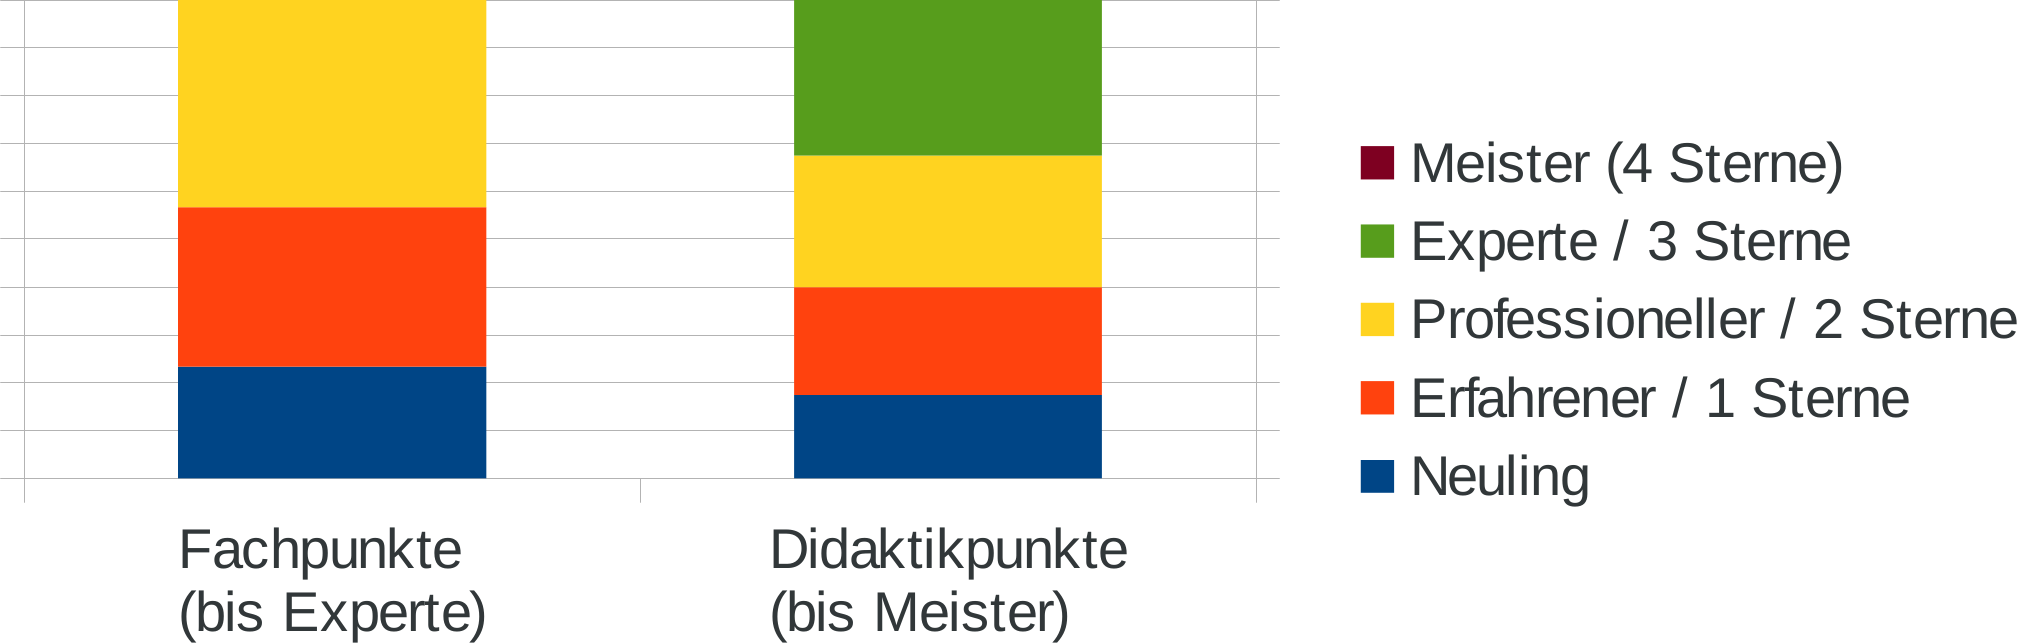
\includegraphics[width=1\textwidth]{verteilungDerPunkte.png}
\caption{Verteilung der Punkte}\label{ref:vertPunkt}
\end{figure}
Ein Meister hat durch das Erhalten der höchsten Wertung für die didaktische
Fähigkeit bereits bewiesen, dass er Spaß an der Vermittlung von Wissen hat.
Demnach bedarf er keiner weiteren Motivation eines höheren Ranges.
Vielmehr möchte er keine negativen Bewertungen seiner Lernenden erhalten und
bemüht sich der weiteren hochwertigen Qualität seiner Lerneinheiten.

\section{Rollen für Anwender}
Passend zum zuvor beschriebenen Konzept werden drei Rollen für Anwender
definiert. Dabei ist das Innehaben mehrerer Rollen zur gleichen Zeit ein Teil
des Modells. Zusammenfassend sind die Rechte und Pflichten eines Nutzers in den
verschieden Rollen in Tabelle \ref{tab:privilegesRoles} aufgeführt. Das dort
aufgeführte Forum ist nicht Teil der ersten produktiven Version (siehe
Abschnitt \ref{ref:weitereIdeen})

\subsection{Administrator}
Der Administrator ist der Verwalter der Plattform und damit für den
reibungslosen Ablauf seitens der Nutzer verantwortlich. Dazu kontrolliert er den
Zusammenhalt des Systems und greift bei inkonsistenzen oder Fehlern ein. Auch
bildet er die Schnittstelle zur Community, die sich in der Weiterentwicklung von
Masterly Mate engagiert.

\subsection{Lernender}
Der Lernende bildet die Hauptzielgruppe des Systems. Er soll WBTs finden, diese
durcharbeiten können und sich an Tutoren wenden, falls er auf ein Problem oder
Unklarheiten stößt. Dazu bietet Masterly Mate ihm das auffinden eines an sein
Fachwissen angepasstes Training. Weiterhin kann er Tutoren kontaktieren, die in
seinem Umkreis wohnen und passend zu seinem Rang Inhalte zu erläutern verstehen.
Die Lokation wird anhand der Postleitzahl festgemacht.

Ein Lernender kann in seinem fachlichen Level bis zum Experten aufsteigen.
Nähere Erläuterungen zu den fachlichen Rängen wurden in Abschnitt
\ref{ref:rankTopic} aufgeführt.

\subsection{Tutor}
Ein Lernender kann ab dem zweiten fachlichen Rang des Dreyfus-Modells (siehe
\ref{ref:dreyfus}) in seinem Profil die Einstellung "`Tutor"' anwählen. Damit
erscheint er unter den Suchergebnissen für Lernende, die einen Tutor suchen. Als
Tutor wird man von Lernenden gefunden, die Unterstützung in einem Fachgebiet
suchen.

\section{Dokumentation der API}
\begin {k}
mit "`rake doc:app"' lässt sich die Dokumentation erstellen

Verfügbar machen mit Link auf "`doc/app/index.html"'

Uebernimmt Julian?
\end{k}

\section{Automatisch generierte Filterung von Ergebnissen}
\begin{k}
\begin{itemize}
  \item Profilinfos werden ausgelesen und zur Eingrenzung der Ergebnisse
  verwendet
  \item daher kein Suchfeld nötig
\end{itemize}
\end{k}
Die Suche von WBTs wird Über reine SQL-Abfragen realisiert. 
Dies bedeutet, dass bei einem Aufruf der WBT-Liste, die Daten des betreffenden Users ausgelesen werden. 
Entsprechend des Levels eines Users im betreffenden Themengebiet werden die
Dafür vorgesehenen WBTs, welche er noch nicht absolviert hat angezeigt. 

\section{Themen}
Die Themen (oder Topics/Themengebiete) grenzen die WBTs voneinander ab und sind
neben den Leveln ein Suchkriterium. Jedes WBT ist Teil mindestens eines
Themengebietes. Außerdem sind die Ränge an die Themen gebunden. Der Benutzer
kann WBTs in jedem Themengebiet absolvieren und im Rang aufsteigen. Dabei ist zu
beachten, dass ein Benutzer einen bestimmten Rang nur in einem Themengebiet
haben kann. Das bedeutet, dass er zwar in einem Gebiet den Status eines
Expertise haben kann, in einem ganz anderen jedoch ein absoluter Newbie ist. Ist
ein WBTs zwei (oder mehr) Themen zugeordnet, so erhält der Benutzer bei
Abschluss die Punkte für beide Themengebiete. Themen können Unterthemen haben,
daher kann ein Benutzer innerhalb eines Überthemas unterschiedliche Ränge haben.
So kann z.B. ein Benutzer im Thema Informatik ein Expertise sein und zugleich in
den Unterthemen Datenstrukturen und Algorithmen Specialist bzw. Newbie sein.
Die Beziehung von Benutzer zu Themengebiet ist m:n, ebenso ist die Beziehung
zwischen Thema und WBT m:n. Die Beziehung von Themen zu ihren Unterthemen ist
1:n. Das hier Beschriebene ist der Stand der Alpha-Version. Eine mögliche
Änderung für die Zukunft wäre, dass erreichte Punkte eines Unterthemas auch im
Überthema gutgeschrieben werden.
	\chapter{Anwenderseite}
Dieses Kapitel zeigt den Teil der Konzeption, der für Anwender sichtbar und
wichtig ist.

\section{Gamification}\label{ref:gamificationConcept}
In Abschnitt \ref{ref:gamification} wurden die wesentlichen Aspekte von
Gamification angesprochen. Hier erfolgt die Konkretisierung derartiger
Eigenschaften in die Konzeption von Masterly Mate.

\subsection{Belohnungskriterien}
Um die Motivation stets auf einem hohen Niveau zu halten, bedient sich Masterly
Mate einer Auswahl an Belohnungskriterien.

Die \textbf{erreichte Punktzahl} im Quiz eines WBTs wird für das Erreichen des
nächst höheren Levels hinzugenommen. Analog dazu erhalten Tutoren
\textbf{Sterne} für qualitativ hohe Unterweisungen. Zuzüglich zu den regulären
Punkten für die fachlichen und den tutoriellen Rang können \textbf{Wertmarken}
gesammelt werden mit denen einem Avatar oder dem \ac{GUI} mehr
Gestaltungsmöglichkeiten verliehen werden.

\subsection{Etappenweise Herausforderungen}
Ein weiteres Mittel, um die Motivation zu fördern sind Spielmechaniken, die in
die Anwendung eingebracht werden. Für diese ist es erforderlich, dass für jede
Art von Nutzer Anreize bestehen. 

Die drei Ränge Neuling, regulärer Nutzer und Enthusiast sind nicht zu
verwechseln mit den Rängen des Dreyfus-Modells aus Abschnitt
\ref{ref:dreyfusConcept}. Die hier betrachteten Ränge in Bezug auf Gamification
berücksichtigen die Handhabe der Software als solche. Ein Neuling verwendet die
Anwendung zum ersten mal oder bisher nur wenige male. Der reguläre Nutzer ist
ein Stammgast der Plattform, während der Enthusiast schier nicht schlafen kann,
ohne die Anwendung täglich verwendet zu haben.

Allen Nutzern ist gemeinsam, dass sie sich selbst gut evaluieren können. Sie
erhalten die Möglichkeit Statistiken einzusehen. Für die erste Version von
Masterly Mate ist eine Art Ladebalken vorgesehen, welcher je nach Füllstand
zeigt, wie groß die Erfüllung der erforderlichen Gesamtpunktzahl für einen Rang
ist. Über seine Wertung kann sich ein Nutzer stets im Feld aller Nutzer
einordnen. Dabei kann jeder für sich individuell entscheiden, ob es für ihn
wichtig ist, in die Top-Ten zu gelangen \cite{grubenMerkeBabics:2012}.

\subsubsection{Neuling}
Als erstmaliger Nutzer einer Plattform oder Anwendung benötigen Neulinge einen
vereinfachten Einstieg und eine leicht verständliche Anleitung. Auch muss die
GUI übersichtlich gestaltet sein, sodass nicht bereits nach wenigen Klicks
Frustration entsteht.

In Masterly Mate wird daher von Beginn an eine Möglichkeit zur
Internationalisierung (siehe Abschnitt \ref{ref:internationalisierung})
umgesetzt. So sieht der Anwender das Interface stets in seiner Sprache der Wahl
und stößt somit nicht auf Verständnisprobleme.

Weiterhin erhält ein neuer Nutzer analog seines fachlichen Rangs Zugang zu
einfachen WBTs, die leicht verständlich sind. Stößt er hier bereits auf
Probleme, so kann er sich einen Tutor zu Rate ziehen
\cite{grubenMerkeBabics:2012}.

Eine Anleitung im Sinne eines Handbuches ist für die erste produktive Version
nicht angedacht.
  
\subsubsection{Regulärer Nutzer}
Nutzer, die die Anwendung in moderater Weise nutzen, sind grundsätzlich
zufrieden mit dem, was ihnen geboten wird. Sie sind aber noch
begeisterungsfähig.

Ein solcher Stammgast kann in Masterly Mate auf noch höhere Ränge aufsteigen,
denn ihm fällt es leichter den in Abschnitt \ref{ref:rankTopic} angesprochenen
jährlichen Test zu bestehen. Als Tutor strebt er eventuell danach ein Meister zu
werden.

Um ein Erlebnis analog des in Abschnitt \ref{ref:basFlow} beschriebenen Flows zu
unterstützen, steigt auch das Niveau der zur Verfügung stehenden WBTs. So kann
der Stammnutzer bei Bedarf stets neue Herausforderungen suchen
\cite{grubenMerkeBabics:2012}.

\subsubsection{Enthusiast}
Ein Enthusiast wird alles daran setzen seinen Experten oder meisterlichen Rang
zu behalten. Er wird also weiterhin Unterweisungen geben und genießt sein
Privileg, WBTs editieren zu können. Je nach Interesse kann er seinen Meister
Rang dazu nutzen in andere Fachgebiete einzusteigen und dort für sämtliche
Mitglieder unterhalb seines zugehörigen fachlichen Rangs mit Rat zur Seite zu
stehen \cite{grubenMerkeBabics:2012}.

\section{Generieren von Motivation}
Zusammen mit der im vorangegangenen Abschnitt beschribenen Konzeption von
Gamification in Masterly Mate wird an dieser Stelle die Integration der in
Abschnitt \ref{ref:basMotivation} beschriebenen Motivation erläutert.

In diesem Abschnitt wird ein Blick auf die motivierenden Merkmale aus
Anwendersicht beschrieben, die im Wesentlichen bereits im vorangegangenen
Abschnitt für die Umsetzung von Gamification besprochen wurden. Dieser wird
separiert in intrisische und extrinsische Motivation dargestellt.

\subsection{Intrinsisch motivierende Aspekte}
Ein Nutzer von Masterly Mate strebt von sich aus nach Weiterbildung und damit
nach einem höheren fachlichen oder didaktischen Rang. Beinahe nebenbei steigt er
dafür immer tiefer in fachliche Themen ein. Für seine Leistungen möchte er
Feedback erhalten und mit gleichgesinnten reden oder helfen. 

Tutoren haben zusätzlich die Möglichkeit ihr Langzeitgedächtnis mithilfe von
immer wiederkehrenden Unterweisungen zu schulen. Damit zusammenhängend
trainieren sie sich in ihren didaktischen Fähigkeiten.
  
\subsection{Weitere extrinsisch motivierende Merkmale}
Zu den intrinsischen Motivatoren kommen weitere extrinsische Motivatoren. Dazu
gehören der Erhalt von Belohnungen, mehr Möglichkeiten in der Gestaltung des
Interfaces oder Avatars oder eine Bestenliste zum Leistungsvergleich mit anderen
Nutzern.

Macht man sich in der Plattform einen Namen als Tutor oder beteiligt sich an
regen Diskussionen im Forum, so erfährt man Lob und Kritik von gleichgesinnten.
Insgesamt lässt Masterly Mate eine persönliche Analyse in Form von Statistiken
zu.
	\part{Implementierung}
	\chapter{Entwurf}\label{ref:chaptScript}
Der in diesem Kapitel beschriebene Entwurf zeigt konkret, wie das Konzept von
Masterly Mate umgesetzt werden wird. Hier werden Schemata und Architekturen
entwickelt, die im Kapitel \ref{ref:chaptImplementation} in Programmcode
umgesetzt werden.

\section{Realisierungsmethodik}
Nachdem in den vorangegangenen Kapiteln das Konzept von Masterly Mate erläutert
wurde, stellt sich die Frage nach einer geeigneten Möglichkeit zur Umsetzung. Da
die Anwendung stets verfügbar, leicht erreichbar, modular und einfach zu
verwalten sein soll, ist \ac{RoR} das Mittel der Wahl. Dieses bietet viele
interessante Features in Form von sogenannten gems, die dank einer regen
Community stets aktualisiert und erweitert werden. Zudem unterstützt es moderne
Programmierparadigmen, wie \ac{DRY} und \ac{KISS}. Dadurch bleibt die Anwendung
aus Sicht der Programmierer übersichtlich und erscheint sehr strukturiert. Das
das Framework der \ac{MVC}-Architektur folgt, schafft einen weiteren Grundstein
zur Trennung von Zuständigkeiten\footnote{bekannter unter "`separation of
concerns"'} und sorgt auch damit für Übersichtlichkeit. 

Weiterhin ist dieses Framework für die Weiterentwicklung im
OpenSource-Bereich prädistiniert, da damit bisher populäre
Webanwendungen, wie Twitter, realisiert wurden.

Darüber hinaus wird darauf geachtet, die Komponenten nach und nach nur dann zu
entwickeln, wenn sie tatsächlich gebraucht werden. Diese Vorgehensweise nach dem
\ac{YAGNI}-Prinzip beugt ein überlaufenes, unübersichtliches und schwer
zu wartendes Produkt vor.

\section{Internationalisierung}\label{ref:internationalisierung}
\begin{k}
Keine Internationalisierung in WBTs! (WBTs brauchen Attribut: Sprache)
Was ist die Default-Language? -> Sprache des Nutzers (User auch Attribut:
Muttersprache oder Herkunftsland)

Uebernimmt Julian?
\end{k}

\section{Beschreibung des Entwurfsklassendiagramms und
Use-Case}\label{ref:classModel}
\begin{k}
\subsection{Use-Case Diagramm}
Im obigen Use-Case Diagramm, sind die enzelnen ben�tigten Komponenten enthalten, wie sie die Analyse ergeben hat. 
Zun�chst einmal lassen sich Aktoren ausmachen, 
welche in System/Software-Aktoren und menschliche Aktoren aufteilen lassen. 
Bei den Softwareseitigen Aktoren ergab die Analyse als Aktoren den Webserver, ein 
Einzelnes WBT (sie sollen nach Abschluss die Punkte im System eintragen), das Autorenwerkzeug und den Webbrowser. 
Auf der Seite der Aktoren lie� sich der Lernende (Standard-User), Tutor, Autor und Admin ermitteln.
Zu beachten ist, dass die Aufteilung der menschlichen Aktoren auch eine Berechtigungshierarchie darstellt, wobei 
ein Lernender die geringsten und ein Admin die meisten Berechtigungen hat. 
Die einzelnen Use Cases werden nun jeweils im folgenden kurz beschrieben. Zu beachtenn ist dabei noch, dass diese 
Analyse sich nicht zwingend mit dem Ergebnis aus der Studienarbeit deckt, 
da Funktionalit�ten auf sp�tere Releases verschoben worden sind.

WBT durcharbeiten
Agierende Aktoren: WBT, Lernender, Tutor, Autor, Admin
Ein Benutzer startet ein WBT und schlie�t es erfolgreich ab bzw. scheitert oder beendet es vorzeitig. 
Im Anschluss daran, werden die erreichten Punkte im System eingetragen.
In der Version der Studienarbeit, wird dies noch vom Benutzer selbst durchgef�hrt. Sp�ter soll dies das WBT �bernehmen.
	
Bewerten
Agierende Aktoren: Lernender, Tutor
Den Use Case Bewerten gibt es in zwei Auspr�gungen. Die erste Auspr�gung ist die Bewertung eines Tutors. 
Hat ein Lernender oder eine anderer Tutor (im folgenden beide als "Lernende" bezeichnet) 
von dem Betreffenden Benutzer Hilfe erhalten, so kann der Lernende im Anschluss daran diese Hilfe im System bewerten. 
Dies kann er mit Sternen und wahlweise mit einem Kommentar tun (Kommentar noch nicht in der
Alpha-Version).
Die Zweite Auspr�gung ist die Bewertung eines WBTs. Ein Benutzer muss das WBT daf�r abgeschlossen haben. 
Ebenso wie beim Tutor kann er dies �ber Sterne und Kommentare tun.
	
Sprache verwalen
Agierende Aktoren: Alle menschlichen Aktoren (Auspr�gung Sprache hinzuf�gen kann nur der Admin)
Ebenso wie im obigen Use Case gibt es hiervon zwei Auspr�gungen. Nummer Eins ist der Use Case Sprache wechseln. 
Dieser kann von jedem Benutzer durchgef�hrt werden und bewirkt, dass alle Zeichenketten in MasterlyMate,
welche in der betreffenden Sprache vorhanden sind, ausgetauscht werden.
Use Case Nummer Zwei kann nur von einem Administrator durchgef�hrt werden. Und bewirkt die Erzeugung einer weiteren Sprache, 
welche eingestellt werden kann. Gegenw�rtig wird dies noch direkt durch 
eine �nderung der Sprachdateiten getan.

Profil verwalten
Agierende Aktoren: Alle menschlichen Aktoren
Auch dieser Use Case verf�gt �ber zwei Auspr�gungen. Der erste Use Case ist das bearbeiten eines Profils. 
Dies kann nur der besitzer des jeweiligen Profils.
Den anderen Use Case kann hingegen jeder Benutzer durchf�hren. Es handelt sich dabei um das Betrachten eines Profils. 
Dies ist insbesondere f�r die Kontaktaufnahme eines Benutzers zu einem Tutor notwendig.

Suchen
Agierende Aktoren: Alle menschlichen Aktoren
Es k�nnen sowohl Tutoren als auch WBTs gesucht werden. Dabei wird jeweils ber�cksichtigt welches Themengebiet gefragt ist.
	
Themengebiet abfragen
Agierende Aktoren: Webserver
Der Webserver �berpr�ft bei einer Suchanfrage die einzelnen Themen.
	
Themen verwalten
Agierende Aktoren: Admin, Webserver
Nur der Admin kann die beiden Auspr�gungen dieses Use Cases durchf�hren, welche das Hinzuf�gen und L�schen eines 
Themas darstellen.
	
WBT verwalten
Agierende Aktoren: Admin, Autor, Webserver
Dieser Use Case besitzt drei Auspr�gungen. Admin und Autor k�nnen WBTs einbinden. Es kann jedoch nur der User, 
welcher ein WBT eingebunden hat, dieses auch wieder entfernen bzw. ersetzen. Dies gilt nicht,
wenn der betreffende Benutzer ein Administrator ist. Dieser kann jedes WBT l�schen oder ersetzen.
	

Entwurfsklassendiagramm

In dem Entwurfsklassendiagramm, sind die Models und ihre Beziehungen zueinander dargestellt. 
Diese Modelle bilden einzelne Konzepte im System ab. 
So stellt User ein Zentrales Modell dar, welches als Abbildung eines Benutzers im System f�r die Authentifizierung 
verantwortlich tr�gt. Au�erdem werden dem User verschiedene Themen und WBTs zugeordnet.
Diese Verbindungen ben�tigen jeweils Assoziationsklassen. Dies liegt daran, dass es in dieser Verbindung 
Attribute gibt, welche sich nicht eindeutig User oder WBT bzw. Thema zuordnen lassen.
Bei der Verbindung User-Thema ben�tigt man ein Attribut f�r die Punkte, welche bisher von dem User in dem System 
erziehlt worden sind. Au�erdem muss klar sein welchen Rang ein User in dem jeweiligen Thema inne hat.
Die Verbindung User-WBT dagegen ben�tigt eine Variable um zu hinterlegen ob ein User das WBT bereits einmal 
abgeschlossen hat und wenn ja, wie viele Punkte er erreicht hat.
Das WBT-Model verf�gt �ber eine ID, sowie �ber einen Pfad zur eigentliche
SCORM-Datei. Wie bereits erw�hnt ist es einem oder mehreren Themen (Topics)
zugeordnet.
\verb+\label{ref:objectWBT}+\label{ref:objectWBT}
\end{k}

\section{Komponenten}
\begin{k}
Struktur hier unklar\ldots noch warten auf die anderen Inhalte von JeyB und
Benni.
\end{k}
Prinzipiell ist Masterly Mate aus zwei Komplexen aufgebaut. Zum einen kann sich
ein Nutzer fachlich weiterbilden. Zum Anderen bietet ein Nutzer als Tutor seine
Hilfe für ein bestimmtes Fachgebiet an.

\subsection{Durcharbeiten von WBTs}

\subsection{Tutorensuche}

\subsection{Navigation, Impressum, Kontakt}
\begin{k}
Uebernimmt Julian
\end{k}

\subsection{Themen}
\begin{k}
Themen fungieren f�r den Benutzer zum Einen als Suchfilter bei der Suche nach
den WBTs. Dies sorgt daf�r, dass der Benutzer ohne umschweife auf WBTs zugreifen
kann, welche f�r ihn interessant sind. Au�erdem dienen Themen dazu, die
unterschiedlichen R�nge, welche ein Benutzer zur selben Zeit in Masterly Mate
haben kann, voneinanderabzugrenzen. Jeder Benutzer kann in einem Thema nur genau
einen Rang inne haben. Umgekehrt kann er jedoch in beliebig vielen Themen einen
Rang haben
\end{k}
	\chapter{Umsetzung}\label{ref:chaptImplementation}

\section{Nutzerverwaltung}\label{ref:sectNutzerverwaltung}
\begin{k}
Im Rahmen dieser Studienarbeit besitzt Masterly Mate neben der Zugangskontrolle
einen eingebauten Mechanismus für die Zugriffskontrolle. Die registrierten
Benutzer werden in der Datenbanktabelle users festgehalten. Diese besitzen neben
dem Attribut Passwort und Benutzername weitere essentielle Attribute wie z.B.
Geburtsdatum, Vorname, Nachname und Geschlecht. Näheres zur Implementierung der
Zugangskontrolle wird im Kapitel \ref{ref:sectAuthentifizierung} erläutert.
Für den Zugriff auf vertrauliche Ressourcen, wie z.B. das Benutzerprofil, die
vom Benutzer durchgeführten Assessments und Examen sowie die zugänglichen WBTs
und die Nutzerstatistik, müssen vor unberechtigten Nutzern geschützt werden.
Für diese Autorisierungsvorgabe wurde das Gem mit dem Namen CanCan
\footnote{https://rubygems.org/gems/cancan} eingesetzt. Dieses Gem ermöglicht
die zentrale Zugriffsverwaltung auf beliebige Ressourcen. Die Klasse Ability des
Gems ist dabei die einzige Klasse die für die Autorisierung von wichtiger
Bedeutung ist. Diese befindet sich nach der Installation von CanCan im
Verzeichnis app/models/. Die Autorisierung auf Ressourcen wird mit Hilfe der
Methoden can? und cannot? realisiert. Diese Methoden erwarten als ersten
Parameter ein vordefiniertes Symbol, welches die Zugriffsart festlegt. Häufige
Zugriffsarten sind z.B. :manage, :destroy, :update, etc. Im Grunde wird hier der Name der
Aktion angegeben, der auf diese Ressource möglich bzw. nicht möglich ist. Bei
dem zweiten Parameter der Methoden can? und cannot? handelt es sich entweder um
den Namen einer Ressource oder einer Instanz einer Ressource. Nutzt man den
Namen einer Ressource, dann bezieht sich die definierte Aktion auf sämtliche
Instanzen dieser Ressource. Im anderen Fall bezieht sich die Aktion nur auf
diese eine Instanz. Die Autorisierung erfolgt in Masterly Mate direkt im
Konstruktor der Ability Klasse. In Masterly Mate wird eine Gruppenbasierte
Rechtevergabe durchgeführt. Mithilfe der Methode group?, welche in der Klasse
des User Models definiert ist, kann man unter Angabe des Namens einer Gruppe,
überprüfen, ob dieser Nutzer der entsprechenden Gruppe zugehört oder nicht.
der Konstruktor der Klasse Ability erwartet eine Instanz von der Klasse
User. Wird dem Konstruktor eine gültige User Instanz übergeben, so wird
mit dieser Instanz weiter operiert. Andernfalls wird eine neue Instanz der
Klasse User erzeugt und als Gastnutzer interpretiert. Dieser würde lediglich
Zugriff auf öffentliche Ressourcen besitzen und könnte sich erst
Authentifizieren, wenn dieser sich registriert hat. Im anderen Fall wird
überprüft ob der aktuelle Nutzer Mitglied der vordefinierten Gruppe
Administrator ist. Wenn dem so ist, dann besitzt der Nutzer sämtliche Rechte auf
alle Ressourcen. Der einzige Vorgang, der auch einem Administrator verwehrt
wird, ist das Entfernen des eigenen Kontos, da ansonsten die Gefahr
besteht, dass kein Administrator in Masterly Mate zur Verfügung steht und das
Entfernen von bestehenden Gruppen. Ein Nutzer der Mitglied der Gruppe Registered
ist, hat die Möglichkeit das eigene Profil und dessen Assessments zu verwalten.
Dabei kann dieser sämtliche Operationen, bis auf das Entfernen des eigenen Profils,
durchführen. Weiterhin besitzen diese Nutzer lediglich einen lesenden Zugriff
auf Themen und einen ausführenden Zugriff auf WBTs.
\end{k}

\section{Lokationen}
Die Angabe von Lokationen bzw. Routen sind für REST-basierte Webanwendungen
unumgänglich. Diese Lokationen werden in RoR in der Datei 
config/routes.rb spezifiziert. Im Kapitel ref{ref:internationalisierung}
wurde erwähnt, wie I18n in Masterly Mate eingesetzt wird. In diesem Kapitel wird der
Zugriff auf eine Sprachdatei durch Lokationen erläutert. In REST-basierten
Webanwendungen gibt es verschiedene Möglichkeiten die gewünschte Sprache über
die URL anzugeben. Dies kann bspw. über einen Parameter in der URL oder
aber gleich unmittelbar vor dem Wurzelverzeichnis in der URL erfolgen. In
Masterly Mate wird letzteres bevorzugt. Für das Setzen des Ländercodes in der
URL wird dem Nutzer ein sogenannter Languge-Switcher angeboten. Dieses wird
durch eine Combobox repräsentiert, mit dessen Hilfe sich der Nutzer eine Sprache
aus der Liste aussuchen kann. Nachdem der Nutzer sich eine Sprache ausgesucht
hat, wird das onChange Event des DOM-Combobox-Elementes ausgelöst und mit Hilfe
eines reguären Ausdrucks der vorhandene Ländercode in der URL durch den
Ländercode der gewählten Sprache ausgetauscht. Die Klasse I18n besitzt das
Attribut locale. Dieses Attribut beinhaltet als Wert den Ländercode der zu
verwendenden Sprache. In der privaten Methode locale_path des Application
Controllers, wird dieses statische attribute gesetzt und die aktuelle URL
entsprechend angepasst. Die Optik des Language Switchers wird in dem partiellen
Layout unter app/views/shared/_language_switcher.html.erb festgelegt und kann
somit in jedem anderen View ohne Probleme eingebunden werden.
\begin{k}

\end{k}

\section{Suche}
\begin{k}
Uebernimmt Julian/Benni?
\end{k}

\section{SCORM}\label{ref:implSCORM}
Die SCORM-Funktionalität wird in dem Objekt "`wbt"' realisiert, welches in
Abschnitt \ref{ref:objectWBT} beschrieben wurde. 

Die darin enthaltene Upload-Methode, die beim Einfügen und Ändern eines WBTs
aufgerufen wird, speichert das WBT auf dem lokalen Speicher des Servers. Dabei
wird das \ac{PIF} mithilfe der Funktionen aus einem
scorm-gem\footnote{Ressource: \url{https://rubygems.org/gems/scorm}} direkt
entpackt. Dabei ist mit der Berücksichtigung der Validierung stets ein Fehler
aufgetreten. Für die erste Version wird daher keine Validierung unterstützt, das
PIF wird ohne Prüfung entpackt (siehe Abschnitt \ref{ref:problems}). Die
Fehlerursache liegt unter Umständen an dem Alter des gems. Eine genauere Betrachtung ist für
spätere Versionen von Masterly Mate angedacht. 

Mit dem Hochladen und Entpacken werden die nötigen Attibute für den Start des
WBT gepflegt. Dies ist zum einen der Paketname selbst und zum anderen der Pfad
zur Start-Datei des Root SCO. In einer start-Methode werden diese Attribute
ausgelesen und das WBT wird in einem neuen Fenster geöffnet. So kann das WBT den
Raum einnehmen, den es braucht. Masterly Mate bleibt damit unabhängig vom Stil
des Autorenwerkzeugs. Für die erste produktive Version fehlt es noch an einem
geeigneten RTE, da dessen Implementierung den Rahmen der vorliegenden Arbeit
sprengen würde. Daher erfolgt die Registrierung des Ergebnisses zunächst durch
eine manuelle Eingabe des Nutzers.

\section{Lizensierung}
Nach den in Abschnitt \ref{ref:freeLicenses} beschriebenen freien Lizenzen und
dem Einbringen der Idee in das Konzept (siehe Abschnitt
\ref{ref:freeLicensesConcept}) wurde für die Zwecke von Masterly Mate auf die
\ac{AGPL} zurückgegriffen. Da diese mit der \ac{GPL} kompatibel ist, wird
eine eventuelle Verbreitung der Software im Sinne von OpenSource möglich.
Darüber hinaus kann das Projekt unter anderen kompatiblen Lizenten verbreitet
werden \cite{fsf:2007}.

Mit der Nutzung der AGPL entsteht die Pflicht, den Quelltext der Anwendung
direkt als Download anzubieten. Dazu wird im Interface Masterly Mate
ein Link auf die GIT-Ressource im Footer angeboten. Zusätzlich wurde, wie bei
allen Lizenzen nötig, in jeder Datei ein Lizenztext vorrangestellt.

\section{Dokumentation}
Wie in Abschnitt \ref{ref:archDoc} beschrieben, wurde mithilfe der Befehlszeile
\textit{rake doc:app} eine Dokumentation der API erstellt und im Footer
mit einem relativen Link auf \textit{doc/app/index.html} referenziert. Die im
Projekt verwendete Version 10.0.2 von rake bedient sich RDoc in der Version
2.12.2 und dem Darkfish Rdoc Generator 3.

Zusammen mit den Anmerkungen im Quelltext entsteht so eine ausführliche
Dokumentation der Fähigkeiten und Schnittstellen. In einem Index über die
Klassen und Module kann gezielt nach bestimmten Funktionsweisen gesucht werden.
Die dazu angebrachten Kurzbeschreibungen und Verweise bieten einen einfachen
Überblick und verhelfen einem interessierten Anwender oder Programmierer zur
Transparenz über die Funktionsweise von Masterly Mate.

Die Dokumentation der API ist in der englischen Sprache gehalten, da diese für
gewöhnlich nicht multilingual geführt wird und Englisch als Sprache für
computerrelevante Themen anerkannt ist.

\section{Gestaltung}
Das Design von Masterly Mate ist in der ersten Version zunächst einmal von
Funktionalität geprägt. Jedoch finden schon einige der weiter oben aufgezählten
gestalterischen Grundkonzepte hier Eingang. So ist es der Erwartungskonformität
geschuldet, dass Navigation und Anzeige sich in optisch voneinander getrennten
Bereichen befinden. Ebenfalls von vielen anderen Seiten bekannt, ist dass
Konzept, die Änderung der Sprach oben rechts und damit abseits von allen anderen
Kontrollen zu platzieren. Die Navigation ist von der Anzeige durch das Gesetz
der Nähe und einen Sichtbaren Trennstrich getrennt. Um eine bessere
Übersichtlichkeit auf den WBTs zu gewährleisten, werden diese Außerdem in einem
neuen Tab geöffnet. Da Masterly Mate als gamifizierte Anwendung nicht vollkommen
auf ein Mindestmaß an ansprechender Optik verzichten kann, ist es in einem
warmen Orange gehalten. Die wenigen anderen Farben sind so gewählt, dass sie
nicht zu sehr in Kontrast zur Hauptfarbe stehen.

\section{Authentifizierung}\label{ref:sectAuthentifizierung}
\begin{k}
Im Kapitel ref{ref:sectNutzerverwaltung} wurde die Umsetzung der Autorisierung
in Masterly Mate erläutert. In diesem Kapitel wird nun die Umsetzung der
Authentifizierung kurz beschrieben. Damit sich ein Nutzer erfolgreich bei
Masterly Mate registrieren und im Anschluss darauf anmelden kann, wird ein
Authentifizierungsmechanismus benötigt, welches sicher und zudem eine geringe
Wartungskomplexität aufweist. Ein Gem, dass diese Voraussetzungen erfüllt, ist
das Ruby eigene Gem mit dem Namen bcrypt-ruby
\footnote{http://bcrypt-ruby.rubyforge.org/}. Dieses Gem nutzt für die
Passwortverschlüsselung einen SHA-Hash und kann daher für den
heutigen Stand der Technik als sicher eingestuft werden. Dieses Gem setzt
außerdem ein User Model voraus, welches zwei String-Attribute besitzt. Eines mit
dem Namen password_digest und eines mit dem Namen username. Die Methode
has_secure_password bildet den Authentifizierungsvorgang auf dieses Model ab und
muss daher in der Klasse User zu Beginn aufgerufen werden. Die Abbildung auf
dieses Model erfolgt durch Hinzugabe einer Methode mit dem Namen authenticate zu
dieser User Klasse. Der Registrierungsvorgang wird von dem User Controller
verwaltet. Der Authentifizierungsvorgang hingegen vom Session Controller. Der
Session Controller ist für die Verwaltung sämtlicher Sitzungen verschiedener Nutzer
zuständig. In der create Action des Session Controllers wird zunächst geprüft,
ob der anfragende Nutzer alle relevanten Informationen zur Authentifizierung
angegeben hat und ob diese Informationen korrekt sind. Diese beiden Vorgänge
werden von der Methode authenticate, welche auf der gefundenen User
Instanz ausgeführt wird, durchgeführt. Als Parameter erwartet diese Methode lediglich
das vom Passwort. War die Authentifizierung erfolgreich, wird der Nutzer auf die
Startseite weitergeleitet und die Nutzer-ID in dem
Sitzungs-Hash zwischengespeichert. Die destroy action wird aufgerufen, sobald
der Nutzer sich abmeldet. Dabei wird einfach die im Sitzungs-Hash gespeicherte
Nutzer-ID auf nil \footnote{äquivalent zu NULL} gesetzt. Der Nutzer wird danach
ebenfalls auf die Startseite weitergeleitet.
\end{k}

\section{Themen}
Der Model Topic, welches die Themen abbildet verfügt über die Attribute name und
parent\_name. Zweiteres dient zur Identifizierung des Überthemas. Die Wahl
dieses Form der Referenz zu verwenden ist der Datenbank geschuldet. Auf diese Weise
liegt der Fremdschlüssel jeweils auf der n-Seite der 1:n Beziehung.
	\part{Reflexion}
	\chapter{Zusammenfassung der Ergebnisse}\label{ref:chaptConclusion}
	\chapter{Fazit und Ausblick}\label{ref:chaptSummary}

\section{Ideen für weitere Versionen}\label{ref:weitereIdeen}
\begin{k}
\begin{itemize}
  \item Nutzer kann eine Liste aller WBTs sehen, die er absolviert hat
  \item Forum
  \item Durchführung von Refactorings für DRY KISS
  \item Profilbild
  \item SCORM RTE implementieren
  \item Mailerfunktionalität
  \item Investierte Zeit mit in das Konzept für Belohnungen einbringen
  \item Am Ende jedes WBT eine Wertung abgeben (zu schwer/zu leicht) -> tendiert
  eine Wertung zu stark in eine Richtung, wird das WBT dem am nächsten passenden
  Rang zugeordnet
  \item Adaptierung von Lerninhalten, wie in \cite{knall:2005}?
  \item SCORM-Player \cite{mitter:2005}
  \item noch Überraschungen mit einbringen? \cite{korte:2009}
\end{itemize}

\subsection{Gamification für Newbies}
\begin{itemize}
    \item Quick-Start Guide (Video-)Instruction, (Video-)Tutorial
    \item Statistical evaluation (Ranking)
    \item Unlock big equipments for the selected design
    \item Possibility of using a Open-ID
    \item Newsletter-Feature
    \item Self-assessment regarding to school grades
  \end{itemize}
  
 \subsection{Gamification für Regulars}
 \begin{itemize}
    \item Collections of Achievements according to the current progression
  \end{itemize}
  
 \subsection{Gamification für Enthusiasten}
 \begin{itemize}
    \item Levels
    \item Dynamic difficulty / i.e. riddles
  \end{itemize}
  
 \subsection{Weitere Möglichkeiten für Gamification}
\begin{itemize}
\item Design Selection (Tamagochi, Avatar)
  \item Assistance possible
  \item Progress bar
  \item status message
  \item discussion room
  \item class room
  \end{itemize}
  
wie schaut das Gamification-Konzept von MM aus? Irgendwie ist Fortschrittsbalken
und Statistik und Möglichkeit als Tutor zu gering bis Meister. Gut ist der
Anreiz, ab Meister WBTs einbringen und editieren zu können. Wie war das mit dem
Avatar oder der UI, die immer besser gestaltet werden kann?

\end{k}

\section{Anschließende Vorhaben}\label{ref:anschlVorh}
\begin{k}
sehen, was wird
\begin{itemize}
  \item wirklich nur in Ausnahmefällen eine DE? (siehe
  \ref{ref:blendedLearning})
  \item (un)populär
  \item neue Verwendungszwecke
  \item nur eine Installation oder mehrere
\end{itemize}

kann mithilfe von Masterly Mate ein idealer Lehrer gefunden werden?
\end{k}
	
	\phantomsection
 	\addcontentsline{toc}{part}{Verzeichnisse}
	% Anhang
	\clearpage
	\pagenumbering{roman}

	% Abbildungsverzeichnis
	\cleardoublepage
	\phantomsection \label{listoffig}
	\addcontentsline{toc}{chapter}{Abbildungsverzeichnis}
	\listoffigures

	%Tabellenverzeichnis
	\cleardoublepage
	\phantomsection \label{listoftab}
	\addcontentsline{toc}{chapter}{Tabellenverzeichnis}
	\listoftables

	% Quellcodeverzeichnis
% 	\cleardoublepage
% 	\phantomsection \label{listoflist}
% 	\addcontentsline{toc}{chapter}{Listings}
% 	\lstlistoflistings

	% Literaturverzeichnis
	\cleardoublepage
	\phantomsection \label{listoflit}
	\addcontentsline{toc}{chapter}{Literaturverzeichnis}
	\bibliographystyle{agsm}
	\bibliography{studArb2Bib}
	
	\appendix
	\chapter*{Anhang}
	\addcontentsline{toc}{part}{Anhang}
	\chapter{Abbildungen}
\chapter{Tabellen}
\chapter{GNU Free Documentation License}
\input{ads/fdl-1.3}
\end{document}